\documentclass[usenames, dvipsnames, 14pt]{beamer}
\usepackage{standalone}
\usetheme{Frankfurt}
\usecolortheme{beaver}

\usepackage[T2A]{fontenc}
\usepackage[utf8]{inputenc}
\usepackage[english,russian]{babel}
\usepackage{amsmath}
\usepackage{booktabs}

\usepackage{graphicx}
\usepackage{amsfonts}
\usepackage{tikz}
\usepackage{soul}
\usepackage{etoolbox}
\usepackage{import}

\usepackage[outdir=./]{epstopdf}

\renewcommand{\le}{\leqslant}                                                    
\renewcommand{\ge}{\geqslant}

\renewcommand{\leq}{\leqslant}
\renewcommand{\geq}{\geqslant}

\renewcommand{\O}{\mathcal{O}}

\DeclareGraphicsRule{*}{mps}{*}{}

\setlength{\parskip}{8pt}

\begin{document}

\title{Открытая олимпиада 2020}
\subtitle{Разбор задач}
\date{Москва, Сочи, 5-7 марта 2020 г.}
\author{}

\frame{\titlepage}

%%%%%%%%%%%%%%%%%%%%%%%%%%%%%%%%%%%%%%%%%%%%%%%%%%%%%%%%%%%%%%%%%%%%%%%%%%%%%%

\section*{A}
\begin{frame}
  \begin{center}
    \LARGE <<Интересные конкурсы>>
  \end{center}

      \begin{center}
      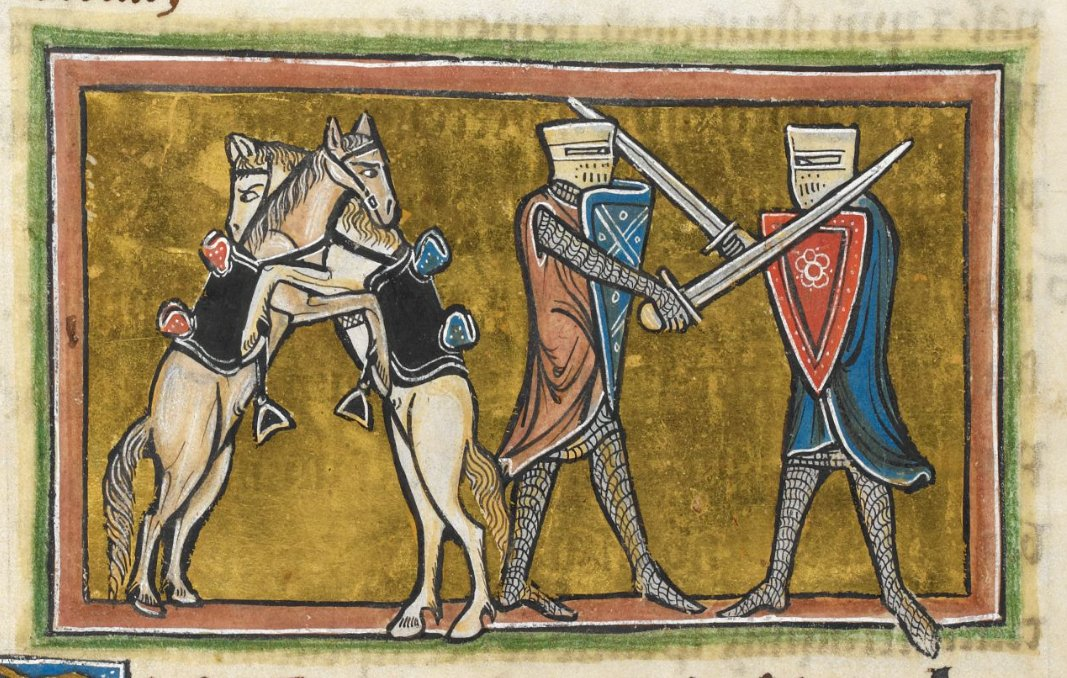
\includegraphics[width=6cm]{memes/a-meme.jpg}
  \end{center}


  \begin{itemize}
  \item Идея задачи --- Григорий Резников, МГУ
  \item Разработка задачи --- Максим Деб Натх, ВШЭ
  \end{itemize}

\end{frame}

\begin{frame}{Постановка задачи}

  \begin{itemize}
  \item Дана скобочная последовательность
  \item За $t$ времени можно перемешать любой её подотрезок длины $t$
  \item Нужно за минимальное время сделать последовательность правильной скобочной
  \end{itemize}
  
\end{frame}

\begin{frame}{Ответ отрицательный}
  \begin{itemize}
  \item Поймём, когда мы не можем сделать последовательность ПСП
  \item Тогда и только тогда, когда число \texttt{<<(>>} и число \texttt{<<(>>} в строке отличается
  \item Иначе всегда можно взять всю строку и переставить в ней за $n$ символы так, чтобы строка стала ПСП, например, \texttt{<<(((($\dots$))))>>}
  \end{itemize}
\end{frame}

\begin{frame}{Основная идея}
  \begin{itemize}
  \item Заметим, что в оптимальном решении отрезки, на которых производятся перемешивания не пересекаются (иначе можно было перемешать сразу нормально)
  \item Значит для перемешивания нужно выбрать набор непересекающихся отрезков.
    \bigskip
  \item Скобочный баланс -- разность между количеством \texttt{<<(>>} и количеством \texttt{<<)>>}
  \item За $bal_i$ ($0 \le i \le n$) обозначим скобочный баланс на первых $i$ символах.
  \end{itemize}
\end{frame}

\begin{frame}{Решение за $\mathcal{O}(n^2)$ (50 баллов)}
  \begin{itemize}
  \item Используем динамику $dp_i=$ сколько времени нужно, чтобы сделать префикс из $i$ символов префиксом ПСП
  \item Если уж перемешивать какой-то отрезок, то его оптимально делать вида <<\t{((\ldots))}>>.
  \item $dp_0 = 0, dp_i = -\infty$, если $bal_i < 0$, иначе

    \[ dp_i = \min \left\{
    \begin{array}{ll}
      dp_{i-1} & \textrm{если } bal_i \geq 0 \\
      j + dp_{i-j} & \textrm{по всем } j \leq i \textrm{ таким, что } \\
      & bal_i \leq bal_{i-j}
    \end{array} \right. \]
  \end{itemize}
\end{frame}

\begin{frame}{Полное решение за $\mathcal{O}(n)$}
  % \begin{itemize}
    %% \item Рассмотрим такой индекс $i$, что что $bal_{i-1} \leq 0$, $bal_{i} < 0$, либо $bal_{i-1} < 0$, $bal_i \leq 0$. Тогда, если символ $s_i$ не будет участвовать ни в одном перемешивании, то итоговая строка будет иметь $i$-й или $i-1$-й префиксный баланс отрицательным
    %%  \item Изобразим данную с.п. как ломанную. Описанные выше индексы~--- это все отрезки ниже линии $x=0$

  Изобразим с.п. графически:

    \begin{figure}[htb]
      \centering
      \resizebox{0.5\textwidth}{!}{
        \begin{tikzpicture}
          \draw [OrangeRed, very thick] (0,0) -- ++(1,-1) -- ++(1, 1);
          \draw [thick] (2,0) -- ++(1,1) -- ++(1,-1);
          \draw [OrangeRed, very thick] (4,0) -- ++(1,-1) -- ++(1, -1) -- ++(1, 1) -- ++(1, -1) -- ++(1, 1) -- ++(1, 1);
          \draw [thick] (-2,0) -- ++(1,1) -- ++(1,-1);
          \draw [green] (-3, 0) -- (+11, 0);
      \end{tikzpicture}}%
      \caption{ПСП до перемешиваний}
    \end{figure}

    Видно, что если взять все последовательности красных скобок и развернуть их, получим ПСП:
    \begin{figure}[htb]
      \centering
      \resizebox{0.5\textwidth}{!}{
        \begin{tikzpicture}
          \draw [blue, thick] (0,0) -- ++(1,1) -- ++(1, -1);
          \draw [thick] (2,0) -- ++(1,1) -- ++(1,-1);
          \draw [blue, thick] (4,0) -- ++(1,1) -- ++(1, 1) -- ++(1, -1) -- ++(1, 1) -- ++(1, -1) -- ++(1, -1);
          \draw [thick] (-2,0) -- ++(1,1) -- ++(1,-1);
      \end{tikzpicture}}%
      \caption{ПСП после перемешиваний}
    \end{figure}
\end{frame} 

\begin{frame}{Полное решение за $\mathcal{O}(n)$}
  \begin{itemize}
  \item При этом каждая из этих скобок должна хотя бы один раз поучаствовать в перемешивании.
  \item Значит, достаточно найти число скобок <<ниже нулевого баланса>>, их количество и будет ответом.
  \end{itemize}
\end{frame} 

\section*{B}
\begin{frame}
  \begin{center}
    \LARGE <<Двойной палиндром>>
  \end{center}

  \begin{center}
      
\includegraphics[width=4cm]{memes/b-meme.jpg}
  \end{center}

  \begin{itemize}
  \item Идея задачи --- Дмитрий Ковальков, ВШЭ
  \item Разработка задачи --- Дмитрий Ковальков, ВШЭ
  \end{itemize}

\end{frame}

\begin{frame}{Постановка задачи}

  \begin{itemize}
  \item Для заданной строки посчитать количество подстрок, являющихся двойными палиндромами
  \item Двойной палиндром --- конкатенация двух палиндромов одинаковой длины
  \end{itemize}
  
\end{frame}

\begin{frame}{Решение за $\O(n^3)$ (19 баллов)}
  \begin{itemize}
  \item Явно переберем все подстроки
  \item Проверим что левая и правая половина являются палиндромами за $O(n)$
  \end{itemize}
\end{frame}

\begin{frame}{Решение за $\O(n^2)$ (33 балла)}
  \begin{itemize}
  \item Проверять что подстрока является палиндромом можно за $O(1)$ с помощью алгоритма Манакера или hash-функции
  \end{itemize}
\end{frame}

\begin{frame}{Полное решение}
  \begin{itemize}
  \item Бывает случай чётной длины палиндрома и нечётной, рассмотрим их отдельно.
  \item Попробуем понять, когда два выбранных центра палиндромов порождают двойной палнидром.
  \item $LCenter$, $RCenter$ --- позиции центров левого и правого палиндромов
  \item $LRadius$, $RRadius$ --- радиусы максимальных палиндромов из позиций LCenter и RCenter
  \item Случаи когда дистанция между центрами нечётна не рассматриваем.
  \end{itemize}
\end{frame}

\begin{frame}{Полное решение}
  \begin{itemize}
  \item Необходимые условия:
  \end{itemize}
  \begin{equation*}
    \begin{cases}
      \frac{RCenter - LCenter}{2} \leq LRadius 
      \\
      \frac{RCenter - LCenter}{2} \leq RRadius
    \end{cases}
  \end{equation*}

  \begin{itemize}
  \item Тогда оба палиндрома достаточно большие, чтобы образовать двойной палиндром.
  \end{itemize}
\end{frame}

\begin{frame}{Полное решение}
  \vspace{-2em}
  \begin{equation*}
    \begin{cases}
      RCenter \leq 2 \cdot LRadius + LCenter & (1)
      \\
      RCenter - 2 \cdot RRadius \leq LCenter  & (2)
      \\
      LCenter < RCenter & (3)
    \end{cases}
  \end{equation*}
  \begin{itemize}
  \item Перебираем $RCenter$, поддерживаем множество $LCenter$, для которых выполнены условия (1) и (3)
  \item Запросы на количество чисел в множестве с условием (2) можно делать с помощью Treap
  \item Итоговая сложность $O(n \log{n})$.
  \item Другое решение: выполнить двумерный запрос на отрезке, можно это делать используя дерево отрезков в offline.
  \end{itemize}
\end{frame}

\section*{C}
\begin{frame}
  \begin{center}
    \LARGE <<Медианный горный хребет>>
  \end{center}

\begin{center}
	
\includegraphics[width=5cm]{memes/c-meme.jpg}
\end{center}

  \begin{itemize}
  \item Идея задачи --- Никита Сендерович
  \item Разработка задачи --- Филипп Грибов
  \end{itemize}

\end{frame}

\begin{frame}{Постановка задачи}

  \begin{itemize}
  \item Дан массив из $n$ чисел, каждое не превышает $a$.
  \item За одну итерацию каждое число массива меняется на медиану из него и двух его окружающих.
  \item Требуется найти значение $c$~--- через сколько итераций числа в массиве перестанут меняться.
  \item Так же надо получить числа массива после $c$ итераций.
  \end{itemize}
  
\end{frame}

\begin{frame}{Решение за $\O(n \cdot c)$ (19 баллов)}
  \begin{itemize}
  \item Будем симулировать процесс, за $\O(n)$ производя по одной итерации.
  \item Так делаем пока массив меняется при очередной итерации.
  \item Так как гарантируется, что $c$ не превышает $10\,000$, то ограничения по времени позволяют это сделать.
  \end{itemize}
\end{frame}

\begin{frame}{Числа не превышают $2$ (24 балла)}
  \begin{itemize}
  \item Если два одинаковых числа стоят подряд в массиве, то они меняться не будут.
  \item Тогда меняться могут только числа внутри отрезков из чередующихся $1$ и $2$.
  \item За одну итерацию концы таких отрезков останутся неизменными, а все числа внутри заменятся на противоположные.
  \item При этом числа рядом с концами отрезков станут равными концам отрезков и в будущем меняться не будут.
  \end{itemize}
\end{frame}

\begin{frame}{Числа не превышают $2$ (24 балла)}
  \begin{itemize}
  \item Итого за одну итерацию длины всех отрезков из чередующихся $1$ и $2$ уменьшаются на $2$.
  \item Тогда общее число итераций равно длине максимального отрезка делённой на $2$.
  \item После всех итераций все числа в левой половине отрезка станут равны левому концу отрезка, а в правой половине~--- правому.
  \end{itemize}

  \begin{center}
    \newcommand{\One} {\textcolor{Orange}{1}}
    \newcommand{\Two} {\textcolor{Magenta}{2}}
    
    \begin{tabular}{cc}
      \textcolor{blue}{11}\Two\One\Two\One\Two\textcolor{blue}{111} & \textcolor{blue}{11}\Two\One\Two\One\textcolor{blue}{22} \\
      \textcolor{blue}{111}\Two\One\Two\textcolor{blue}{1111} & \textcolor{blue}{111}\Two\One\textcolor{blue}{222} \\
      \textcolor{blue}{1111}\Two\textcolor{blue}{11111} & \textcolor{blue}{11112222} \\
      \textcolor{blue}{1111111111} &   \\
  \end{tabular}
  \end{center}
  
\end{frame}

\begin{frame}{Решение за $\O(n \cdot a)$ ($14 + 38$ баллов)}
  \begin{itemize}
  \item Заффиксируем некоторое число $x$ и заменим числа, $< x$, на $1$, а числа $\ge x$ на $2$.
  %% \item Тогда если применить к исходному массиву одну итерацию, и потом заменить на $1$ и $2$ по тому же принципу, получится новый массив с применённой итерацией.
    %% \item Для нового массива мы знаем через сколько итераций он меняться перестанет. Ровно через это количество итераций числа, меньшие $x$, навсегда останутся меньше $x$, а остальные навсегда останутся больше или равны $x$.
  \item Тогда если решить задачу для этого массива, то число $1$ будет означать, что в исходной версии
    в этом месте будет число $< x$, а $2$, что число $\ge x$.
  \end{itemize}
\end{frame}

\begin{frame}{Решение за $\O(n \cdot a)$ ($14 + 38$ баллов)}
  \begin{itemize}
  \item Переберём все возможные $x$ от $1$ до $a$.
  \item Заменим на массив из $1$ и $2$ (по тому же принципу) и посчитаем число итераций, после которых новый массив перестанет меняться.
  \item Максимальное из этих количеств итераций по всем $x$ и будет $c$.
  \item Итого асимптотика $\O(n \cdot a)$.
  \item Чтобы восстановить массив достаточно для каждого элемента массива найти самый большой $x$, что симуляция с этим $x$ всё ещё приводит к ``2''.
  \end{itemize}
\end{frame}

%% \begin{frame}{Решение за $\O(n \cdot a)$ ($14 + 38$ баллов)}
%%   \begin{itemize}
%%   \item Возьмём $x = a$.
%%   \item Заменим числа, меньшие $x$, на $1$, а остальные на $2$.
%%   \item Для нового массива мы знаем, на каких позициях в конце стоит $2$.
%%   \item На этих же позициях в исходном массиве в конце стоят числа, равные $a$.
%%   \end{itemize}
%% \end{frame}

%% \begin{frame}{Решение за $\O(n \cdot a)$ ($14 + 38$ баллов)}
%%   \begin{itemize}
%%   \item Возьмём $x = a - 1$.
%%   \item Аналогично предыдущему поймём, на каком множестве позиций в конце стоят числа, большие или равные $a - 1$.
%%   \item Мы знаем на каких позициях стоят числа, равные $a$.
%%   \item Тогда на всех остальных позициях этого множества будут стоять числа, равные $a - 1$.
%%   \end{itemize}
%% \end{frame}

%% \begin{frame}{Решение за $\O(n \cdot a)$ ($14 + 38$ баллов)}
%%   \begin{itemize}
%%   \item Аналогичные образом поймём на каких позициях стоят числа $a - 2, a - 3, \ldots, 1$.
%%   \item Так получим массив после $c$ итераций.
%%   \item Восстановление позиций одного числа работает за $\O(n)$.
%%   \item Итого асимптотика $\O(n \cdot a)$.
%%   \end{itemize}
%% \end{frame}

%% \begin{frame}{Нахождение $c$ ($28$ баллов)}
%%   \begin{itemize}
%%   \item Из предыдущих слайдов мы знаем, что чтобы найти $c$, можно перебрать все возможные $x$ от $1$ до $a$
%%   \item При каждом $x$ заменить все числа, меньшие $x$, на $1$, а остальные на $2$.
%%   \item В таких новых массивах взять максимальное число итераций, при которых происходят изменения.
%%   \item То есть во всех таких массивах найти самый длинный отрезок из чередующихся $1$ и $2$ и разделить его длину на $2$.
%%   \end{itemize}
%% \end{frame}

\begin{frame}{Нахождение $c$ ($+14$ баллов)}
  \begin{itemize}
  \item Нетрудно показать, что стоит рассматривать только те $x$, которые равны числам массива.
  \item Хотим понять сколько максимум итераций понадобится. Но число итераций при конкретном $x$ равно 0.5 длины
    самого длинного чередующегося отрезка.
  \item Отсортируем все числа массива и будем рассматривать их как $x$ в порядке убывания.
  \item Изначально сделаем $x$ равным \t{max} числу массива и заведём массив из $1$ и $2$.
  \item Далее будем постепенно уменьшать $x$ и пересчитывать $1-2$-отрезки.
  \end{itemize}
\end{frame}

\begin{frame}{Нахождение $c$ ($+14$ баллов)}
  \begin{itemize}
  \item Будем хранить все чередующиеся $1-2$-отрезки в \t{set}.
  \item Как этот \t{set} меняется при уменьшении $x$? Предположим на некоторой позиции $p$ нужно заменить $1 \to 2$.
  \item В случае, если на позиции $p - 1$ находится $1$, нужно объединить отрезок с $p$ с отрезком слева, содержащим $p - 1$.
  \item В противном случае нужно наоборот разделить этот отрезок по позиции $p$.
  \item Аналогично с позицией $p + 1$.
  \end{itemize}
\end{frame}

\begin{frame}{Нахождение $c$ ($+14$ баллов)}
  \begin{itemize}
  \item Так как все отрезки хранятся в $set$, то создание или удаление отрезков работает за $\O(\log n)$.
  \item Так как на каждой позиции изменение $1$ на $2$ происходит ровно один раз, то асимптотика $\O(n \log n)$.
  \item После того как пересчитали отрезки для нового $x$, пересчитываем ответ относительно новых длин.
  \item Нам осталось только получить сам массив после $c$ итераций.
  \end{itemize} 
\end{frame}

\begin{frame}{Полное решение (100 баллов)}
  \begin{itemize}
  \item Будем так же уменьшать $x$ и пересчитывать отрезки из чередующихся $1$ и $2$.
  \item Будем в \t{set} хранить позиции, на которых числа в итоговом массиве пока не известны.
  \item После рассмотрения очередного $x$ научимся понимать, на каких позициях будут стоять числа, равные $x$.
  \item Это те позиции, в которых после $c$ итераций написано $2$ и они ещё не удалены из \t{set}
  \end{itemize}
\end{frame}

%%%

\begin{frame}{Полное решение (100 баллов)}
  \begin{itemize}
  \item После уменьшения $x$ некоторые отрезки останутся прежними, а некоторые изменятся.
  \item На отрезках, которые останутся прежними, не могут появиться новые позиции, про числа на которых мы раньше не знали.
  \item Для каждого изменившегося отрезка поймём во что они превратятся, исходя из их длин и чисел по краям.
  \item Если этот изменившийся отрезок порождает какой-то подотрезок с двойками, то извлечём из \t{set} все ещё не удалённые элементы на этом подотрезке и запишем для них ответ.
  \end{itemize}
\end{frame}

\begin{frame}{Полное решение (100 баллов)}
  \begin{itemize}
  \item Получилось решение за $\O(n \log n)$, можно решить задачу за $\O(n)$.
  \end{itemize}
\end{frame}

%% \begin{frame}{Полное решение (100 баллов)}
%%   \begin{itemize}
%%   \item Для отрезка из чередующихся $1$ и $2$ в конце $2$ будут стоять на некотором подотрезке.
%%   \item Для изменившегося отрезка из $1$ и $2$ найдём такой подотрезок.
%%   \item На этом подотрезке посмотрим на все позиции, про которых числа в итоговом массиве пока не известны.
%%   \item Теперь известны, на них стоит $x$.
%%   \end{itemize}
%% \end{frame}

%% \begin{frame}{Полное решение (100 баллов)}
%%   \begin{itemize}
%%   \item Для каждой позиции она не более одного раза входит в такой подотрезок, после чего навсегда удаляется из $set$.
%%   \item Тогда итоговая асимптотика $\O(n \log n)$.
%%   \item Существует так же решение за $\O(n)$.
%%   \end{itemize}
%% \end{frame}

\section*{D}
\begin{frame}
  \begin{center}
    \LARGE <<Разработка тарифов>>
  \end{center}

  \begin{center}
      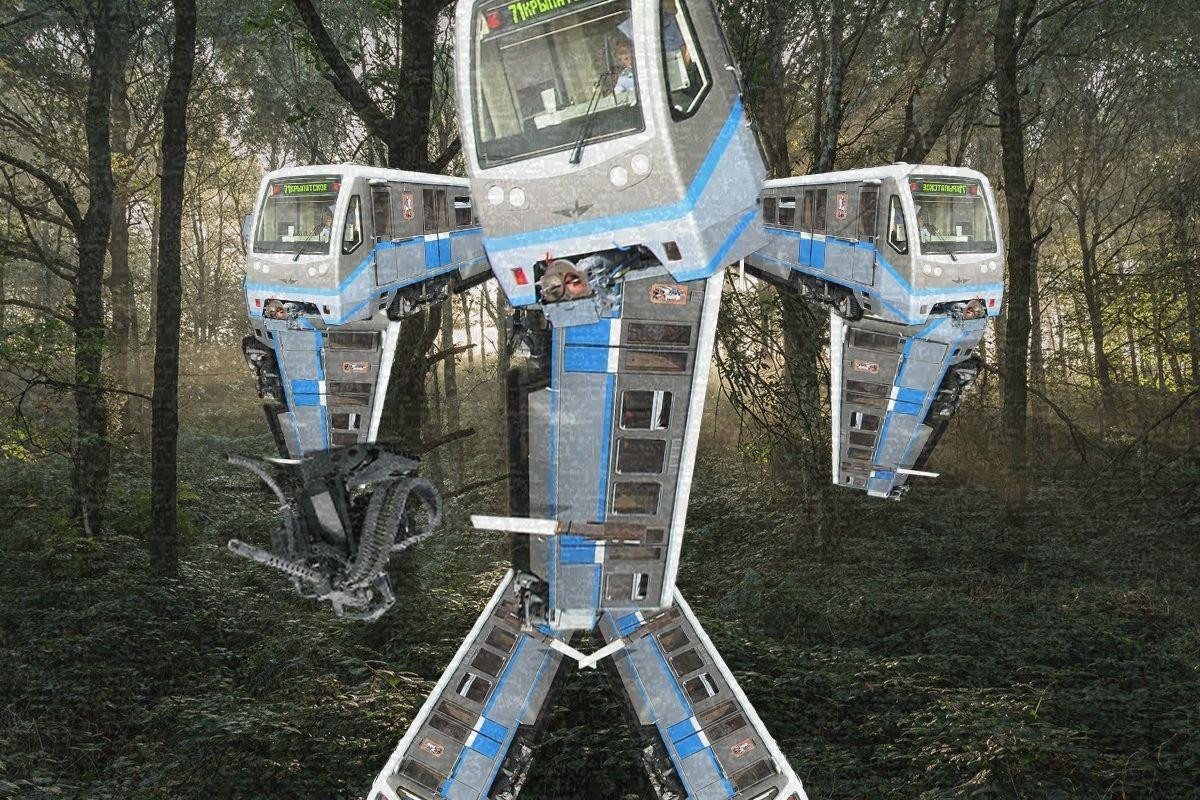
\includegraphics[width=5cm]{memes/d-meme.jpg}
  \end{center}

  \begin{itemize}
  \item Идея задачи --- Григорий Резников, МГУ
  \item Разработка задачи --- Константин Амеличев, ВШЭ
  \end{itemize}

\end{frame}

\begin{frame}{Постановка задачи}

  \begin{itemize}
  \item Дано дерево на $n$ вершинах и $m$ путей
  \item Требуется задать каждой вершине цвет $c_v$
  \item Вдоль пути цвета должны быть расположены монотонно
  \item Максимальное из чисел должно быть как можно меньше
  \end{itemize}

\end{frame}

\begin{frame}{Решение за $\O(n^n \cdot nm)$ (5 баллов)}
  \begin{itemize}
  \item Если раскраска существует, то она существует и с цветами от 1 до $n$
  \item Переберем все раскраски и проверим, что числа вдоль путей возрастают
  \end{itemize}
\end{frame}
\begin{frame}{Решение за $\O(2^n \cdot nm)$ (15 баллов)}
  \begin{itemize}
  \item Разделим ребра на покрытые и не покрытые путями
  \item Ребра второго типа разбивают задачу на несколько меньших задач
  \item Ребра первого типа задают сравнение --- либо $c_v < c_u$, либо $c_u < c_v$
  \end{itemize}
\end{frame}
\begin{frame}{Решение за $\O(2^n \cdot nm)$ (15 баллов)}
  \begin{itemize}
  \item Переберем все возможные сравнения
  \item Рассмотрим вершины в порядке топологической сортировки
  \item Задаем вершине минимальный доступный цвет
  \item Проверяем, что раскраска корректна
  \end{itemize}
\end{frame}

\begin{frame}{Граф --- звезда (10 баллов)}
  \begin{itemize}
  \item Длина каждого пути не больше 3
  \item Построим граф на путях
  \item Проведем ребро между двумя путями, если они не вложены и пересекаются
  \end{itemize}
\end{frame}

\begin{frame}{Граф --- звезда (10 баллов)}
  \begin{itemize}
  \item Выбор направления пути задает направление всей компоненте
  \item Граф должен быть двудольным!
  \item Если граф двудольный, то существует раскраска с максимальным цветом не больше 3
  \end{itemize}
\end{frame}

\begin{frame}{Пути не пересекаются, $\O(n \log C \log n)$ (10 баллов)}
  \begin{itemize}
    \item Раскраска точно существует
    \item Сделаем бинарный поиск по максимальному цвету
    \item Проверим, возможно ли раскрасить дерево в $k$ цветов
  \end{itemize}
\end{frame}

\begin{frame}{Пути не пересекаются, $\O(n \log C \log n)$ (10 баллов)}
  \begin{itemize}
    \item Динамическое программирование по поддеревьям
    \item $dp[v]$ --- минимальный возможный цвет, в который можно покрасить $v$, согласованный с поддеревом
    \item Для определенности считаем, что ребро $v \rightarrow parent_v$ направлено так, что $c_v < c_{parent_v}$
    \item В силу симметрии максимально возможный цвет, если $c_v > c_{parent_v}$ равен $k + 1 - dp[v]$
  \end{itemize}
\end{frame}

\begin{frame}{Пути не пересекаются, $\O(n \log C \log n)$ (10 баллов)}
  \begin{itemize}
    \item Для вершины $v$ есть набор ограничений
    \item Если через $v$ идет вертикальный путь из поддерева $u$, тогда $dp[v] \ge dp[u] + 1$
    \item Если через $v$ проходит путь из поддерева $a$ в поддерево $b$, тогда:
    \begin{enumerate}
        \item $dp[v] \ge dp[a] + 1$
        \item $dp[v] \le k - dp[b]$
    \end{enumerate}
    \item Но мы не знаем, в какую сторону направлен путь
  \end{itemize}
\end{frame}

\begin{frame}{Пути не пересекаются, $\O(n \log C \log n)$ (10 баллов)}
  \begin{itemize}
    \item Попробуем и так, и так
    \item $dp[v] \in [dp[a] + 1, k - dp[b]]$ или $dp[v] \in [dp[b] + 1, k - dp[a]]$
    \item Для каждого пути выпишем два отрезка, и сделаем сканлайн
    \item Найдем самую первую точку, покрытую отрезками всех цветов
    \item Решение за $\O(n \log C \log n)$
  \end{itemize}
\end{frame}

\begin{frame}{Пути не пересекаются, $\O(n \log C)$ (20 баллов)}
  \begin{itemize}
    \item Заметим, что мы взяли ограничения в два множества --- $L$ и $R$
    \item $max(L) + 1 \le min(k - R) \rightarrow max(L) + max(R) \le k - 1$
    \item $dp[v] = max(L) + 1$
    \item Надо разложить пары $dp[a_i],\,dp[b_i]$ по двум множествам
  \end{itemize}
\end{frame}

\begin{frame}{Пути не пересекаются, $\O(n \log C)$ (20 баллов)}
  \begin{itemize}
    \item Зафиксируем, что будет больше --- $max(L)$ или $max(R)$
    \item Тогда в каждой паре разложение определится однозначно --- максимум пойдет в то множество, где максимум больше
    \item Проверим оба варианта на условие $max(L) + max(R) \le k - 1$ и возьмем наилучший
  \end{itemize}
\end{frame}

\begin{frame}{Полное решение (100 баллов)}
  \begin{itemize}
    \item Как в графе-звездочке, строим новый граф
    \item Для каждого ребра становится известен класс эквивалентности
    \item Внутри классов эквивалентности мы знаем ориентацию ребер, относительно <<основного>> ребра внутри класса
  \end{itemize}
\end{frame}

\begin{frame}{Полное решение (100 баллов)}
  \begin{itemize}
    \item Бинарный поиск по ответу
    \item Аналогичная $dp[v]$
    \item Теперь вместо пары $a, b$ у нас будет два множества $A, B$. Внутри такого множества надо будет брать те $a,\,b$ что $dp[a] \ge dp[a'],\ dp[b] \ge dp[b']$.
    \item Свели к предыдущей задаче. В зависимости от подсчета динамики получаем решения за $\O(n \log C \log n)$ или $\O(n \log n)$
  \end{itemize}
\end{frame}


\section*{E}
\begin{frame}
  \begin{center}
    \LARGE <<Глиноведение>>
  \end{center}
  
  \begin{center}
      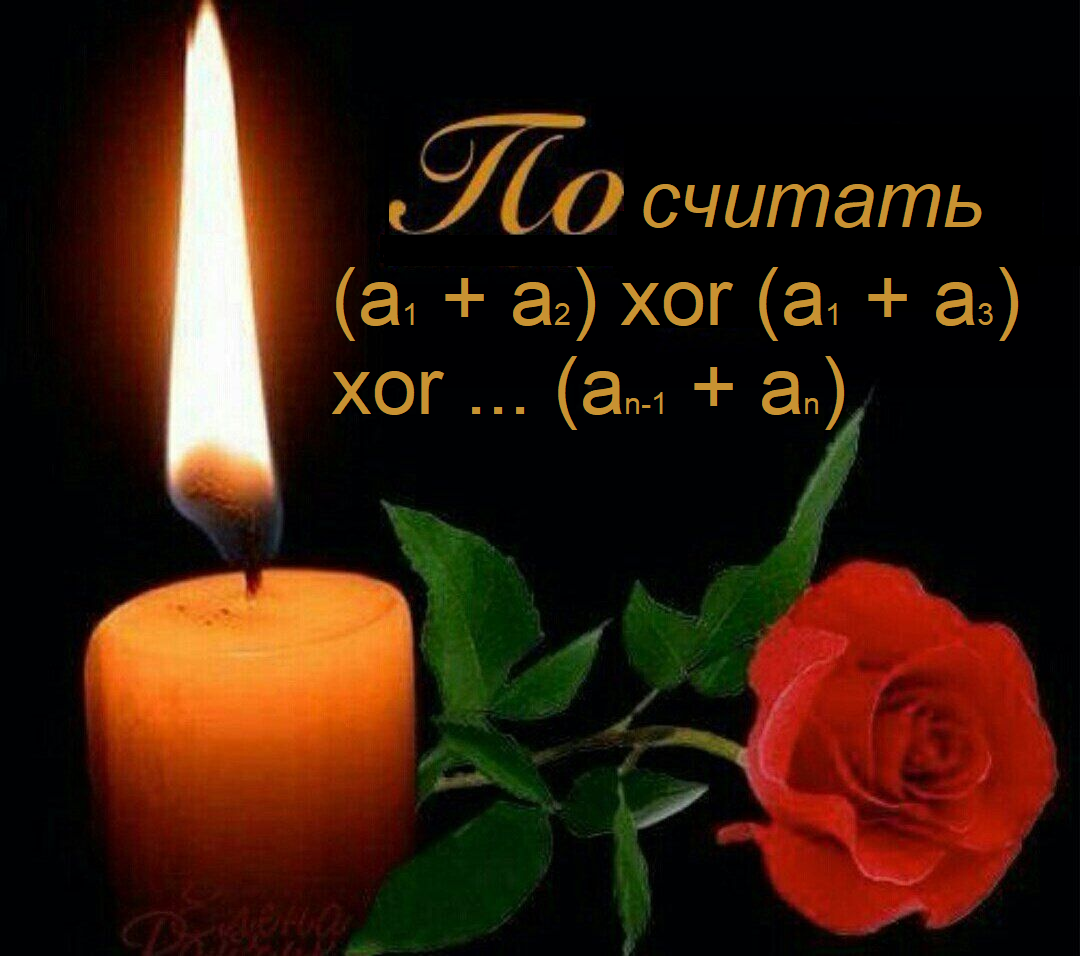
\includegraphics[width=5cm]{e-meme.png}
  \end{center}

  \begin{itemize}
  \item Идея задачи --- Грикукан
  \item Разработка задачи --- Александр Курилкин
  \end{itemize}

\end{frame}

\begin{frame}{Постановка задачи}

  \begin{itemize}
  \item Дан массив чисел, нужно посчитать побитовый xor сумм всех пар чисел в нем
  \end{itemize}

\end{frame}

\begin{frame}{Решение за $\O(n^2)$ (15 баллов)}
  \begin{itemize}
  \item Двойным for явно переберем все пары и посчитаем ответ.
  \end{itemize}
\end{frame}

\begin{frame}{Решение за $\O(n + C^2)$ (20 баллов)}
  \begin{itemize}
  \item Посчитаем количество каждого числа;
  \item После этого двойным for переберем все возможные пары значений чисел;
  \item Пусть значения равны $i$ и $j$;
  \item Если $i \neq j$, то если $cnt_i \cdot cnt_j \bmod 2 = 1$, то $i + j$ войдет в считаемое выражение нечетное кол-во раз, и его нужно учесть (проксорить $ans$ с $i + j$), иначе нет;
  \item Если $i = j$, то делаем все то же, только теперь кол-во раз, которое $i + i$ войдет в выражение, считается по формуле $\frac{cnt_i \cdot (cnt_{i} - 1)}{2}$.
  \end{itemize}
\end{frame}

\begin{frame}{Полное решение}
  \begin{itemize}
      \item Будем считать каждый бит в ответе отдельно. Пусть мы хотим посчитать, чему равен $k$-й (в 0-индексации) бит;
      \item Заметим, что тогда от чисел нас интересуют только их биты от $0$-го до $k$-го, то есть можно взять все числа по модулю $2^{k + 1}$;
      \item Теперь сумма двух чисел может не превышать $2^{k + 2} - 2$, при этом $k$-й бит равен 1, если эта сумма попадает в отрезок от $[2^k; 2^{k + 1})$ или $[2^{k + 1} + 2^k; 2^{k + 2} - 2]$.
  \end{itemize}
\end{frame}

\begin{frame}{Полное решение}
  \begin{itemize}
      \item Осталось посчитать кол-во пар чисел, дающих такую сумму. Для отсортируем все взятые по модулю $2^k$ числа и пройдемся двумя указателями или сделаем бинпоиски для каждого числа;
      \item Итоговое время работы: $O(n \log n \log C)$;
      \item Бонус: можете убрать $\log n$ из асимптотики?
  \end{itemize}
\end{frame}

\section*{F}
\begin{frame}
  \begin{center}
    \LARGE <<Глиноведение>>
  \end{center}

  \begin{itemize}
  \item Идея задачи --- Кто-то
  \item Разработка задачи --- Кто-то
  \end{itemize}

\end{frame}

\begin{frame}{Постановка задачи}

  \begin{itemize}
  \item Лалала
  \end{itemize}
  
\end{frame}

\begin{frame}{Решение за $\O(max(x, y))$ (50+ баллов)}
  \begin{itemize}
  \item Лалала.
  \end{itemize}
\end{frame}

\begin{frame}{Полное решение}
  \begin{itemize}
  \item Лалала
  \end{itemize}
\end{frame}

\section*{G}
\begin{frame}
  \begin{center}
    \LARGE <<Реалити-шоу>>
  \end{center}

  \begin{center}
      
\includegraphics[width=5cm]{g-meme.jpg}
  \end{center}

  \begin{itemize}
  \item Идея задачи --- Романов Владимир, ВШЭ
  \item Разработка задачи --- Погодин Михаил, ВШЭ
  \end{itemize}

\end{frame}

\begin{frame}{Постановка задачи}
  \begin{itemize}
  \item Даны $n$ значений $v_i \leq m$, $n$ значений $s_i$ и $n + m$ значений $c_i$
  \item Требуется выбрать подмножество индексов $1 \leq i_1 < i_2 < ... < i_k \leq n, v_{i_1} \geq v_{i_2} \geq ... v_{i_k}$ с максимальной стоимостью
  \item При добавлении в множество элемента со значением $v$ в стоимость множества добавляется $c_v$ и если в множестве два элемента со значением $v$, то они оба удаляются и $v + 1$.
  \item Для получения итоговой стоимости нужно вычесть $s_{i_1} + s_{i_2} + ... + s_{i_k}$
  \end{itemize}
\end{frame}

\begin{frame}{Решение за $\O(2^n n^2)$ (14 баллов)}
  \begin{itemize}
  \item Переберем за $\O(2^n)$ подмножество элементов
  \item Далее за $\O(n^2)$ можно просимулировать процесс и найти прибыль
  \end{itemize}
\end{frame}

\begin{frame}{Решение за $\O(n^2)$ для $m = 1$ (24 баллов)}
  \begin{itemize}
  \item В данной группе нужно заметить, что всегда лучше брать людей, которые требуют меньшую зарплату 
  \item Отсортируем работников по возрастанию зарплаты 
  \item Переберем число людей, которых мы возьмем и честно просимулируем
  \end{itemize}
\end{frame}

\begin{frame}{Ключевая идея}
  \begin{itemize}
  \item Перефразируем происходящее 
  \item Представим все элементы как степени двойки
  \item Будем хранить сумму взятых элементов
  \item Мы платим за взятие элемента, прибавляем его к текущему числу и получаем прибыль за какждый перенос
  \end{itemize} 
\end{frame}

\begin{frame}{Решение за $\O(n^22^mm)$ (34 баллов)}
  \begin{itemize}
  \item Сумма взятых элементов не больше, чем $n2^m$
  \item Тогда можно применить метод динамического программирования и
  решить задачу за $O(n^22^mm)$
  \end{itemize}
\end{frame}

\begin{frame}{Решение за $\O(n^2m)$ (75 баллов)}
  \begin{itemize}
  \item Рассмотрим сумму и минимальное число, которое мы взяли
  \item Заметим, что если брать только элементы с таким же значением, то $\log(n)$ бит могут изменится как угодно, а еще возможно будет один перенос вне этих битов
  \item Снова применим метод динамического программирования и попытаемся учесть предыдущее наблюдение
  \end{itemize}
\end{frame}

\begin{frame}{Решение за $\O(n^2m)$ (75 баллов)}
  \begin{itemize}
  \item $dp[value][carry][mask]$, где:\\
  \indent $value$ --- значение возможного нового элемента\\
  \indent $carry$ --- будет ли перенос\\
  \indent $mask$ --- последние $\log(n)$ бит\\
  \item Можно пересчитать $dp[value + 1]$ через $dp[value]$
  \item Итогo мы $n$ раз пересчитаем динамику размером $O(nm)$
  \end{itemize}
\end{frame}

\begin{frame}{Полное решение $\O(n(n + m))$}
  \begin{itemize}
  \item Заметим, что после взятия элемента могут изменится лишь $O(n + \frac{n}{2} + \frac{n}{4} + \ldots) = O(n)$ значений динамики
  \end{itemize}
\end{frame}

\section*{H}
\begin{frame}
  \begin{center}
    \LARGE <<Латинский квадрат>>
  \end{center}
  \begin{center}
      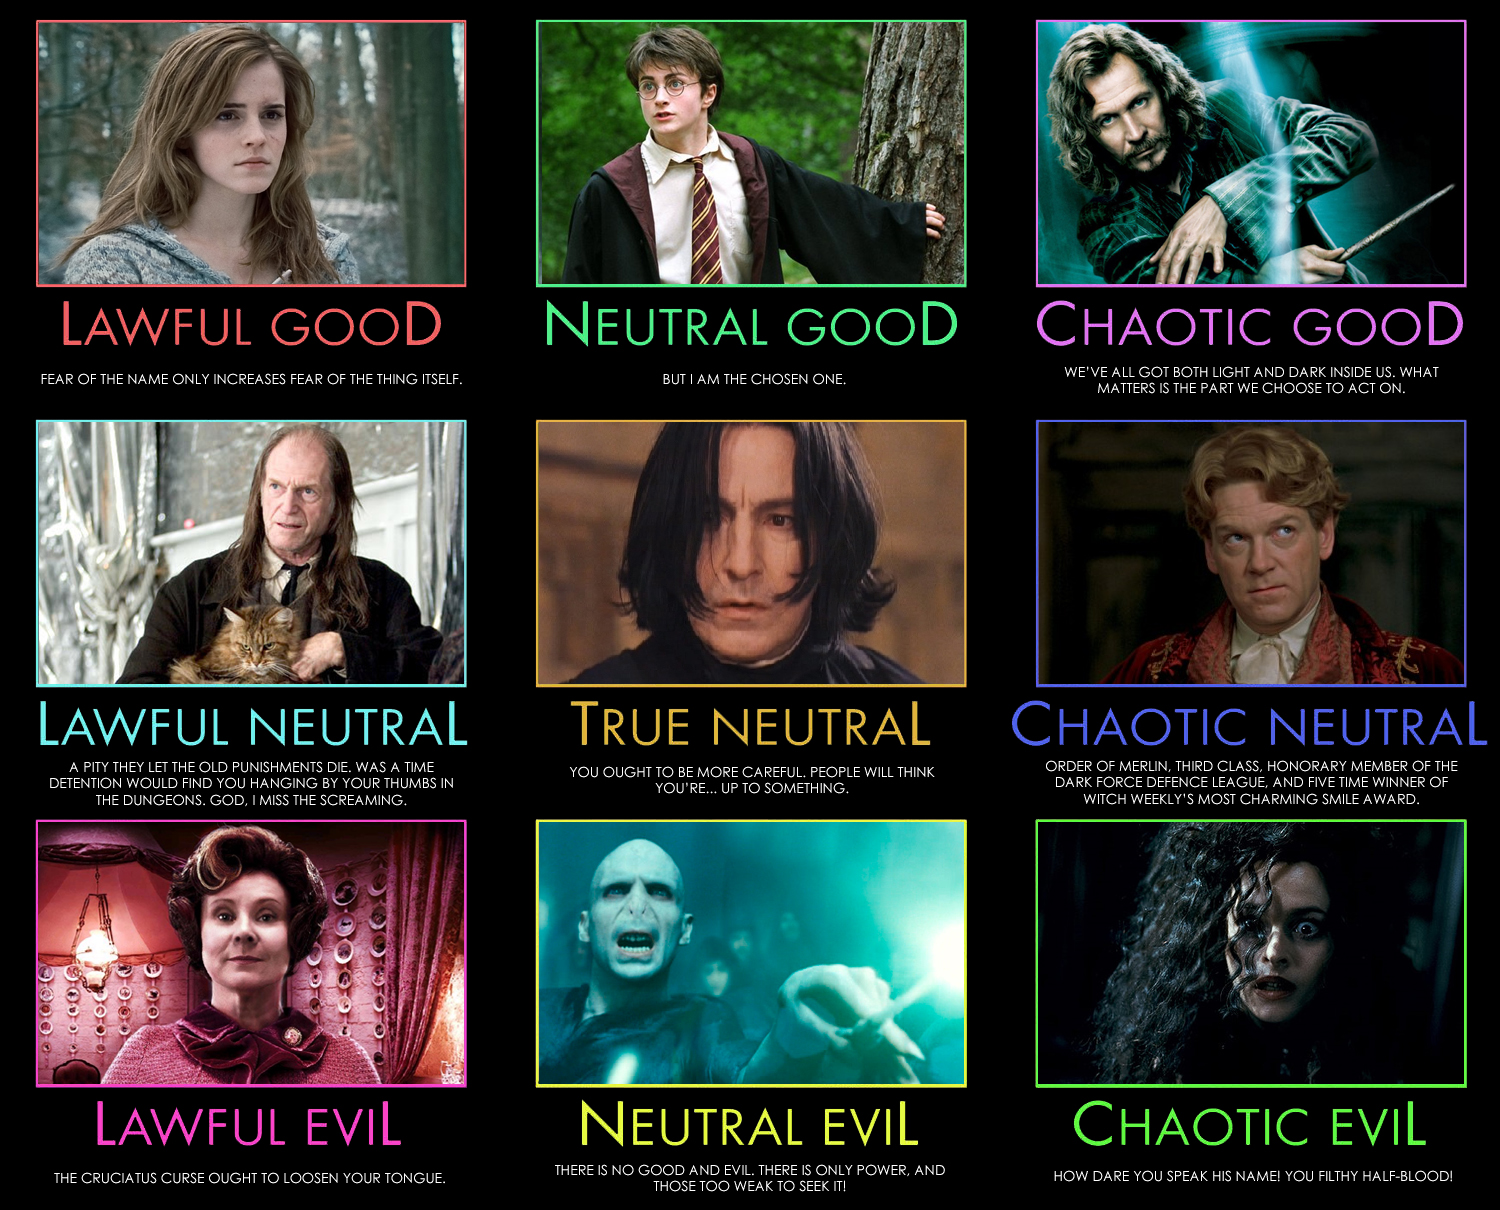
\includegraphics[width=5cm]{memes/h-meme.jpg}
  \end{center}
  \begin{itemize}
  \item Идея задачи --- Михаил Тихомиров, МФТИ
  \item Разработка задачи --- Николай Будин, ИТМО
  \end{itemize}
\end{frame}

\begin{frame}{Постановка задачи}

  \begin{itemize}
  \item Дана матрица $n \times m$.
  \item Нужно найти количество подматриц, которые являются латинскими квадратами.
  \item Латинский квадрат~--- матрица $k \times k$, в которой ровно $k$ различных элементов и в каждой строке и каждом столбце элементы не повторяются.
  \end{itemize}
  
\end{frame}

\begin{frame}{Решение за $\O(n ^ 5)$ (9 баллов)}
  \begin{itemize}
  \item Переберем подматрицу, являющуюся квадратом.
  \item Проверим, что подматрица является латинским квадратом за её размер.
  \item В зависимости от используемых для проверки структур данных, асимптотика может дополнительно умножиться на логарифм.
  \end{itemize}
\end{frame}

\begin{frame}{Решение за $\O(n ^ 4)$ (19~баллов)}
  Сделаем наблюдение:
  
  \begin{itemize}
  \item Квадратная подматрица является латинским квадратом, если:
  \begin{itemize}
  \item В каждой строке и каждом столбце все элементы различны,
  \item Количество различных элементов в подматрице равно длине её стороны.
  \end{itemize}
  \end{itemize}
\end{frame}

\begin{frame}{Решение за $\O(n ^ 4)$ (19~баллов)}
  \vspace{-0.7em}
  \begin{itemize}
  \item Зафиксируем верхний левый угол латинского квадрата.
  \item Будем перебирать длину стороны квадрата в порядке возрастания.
  \item При увеличении стороны на $1$, добавляем новые элементы и проверяем, что не появилось дубликатов в какой-то строке или столбце.
    Также поддерживаем число различных в текущем квадрате.
  \item Для этого для каждой строки, столбца и всего квадрата храним \t{set} или \t{hashset}.
  \item Для фиксированного верхнего левого угла решение работает за $\O(n \cdot m)$
  \end{itemize}
\end{frame}

%% \begin{frame}{Решение за $\O(n ^ 4)$ (19~баллов)}
%%   \begin{itemize}
%%   \item Будем поддерживать количество различных элементов в текущем квадрате
%%   \item Для этого нужно увеличивать счётчик на $1$, когда мы впервые встретили какой-то элемент
%%   \end{itemize}
%% \end{frame}

\begin{frame}{Решение за $\O(n ^ 3)$ (44~балла)}
  \begin{itemize}
  \item Научимся за $\O(1)$ проверять что повторений в строках и столбцах нет.
  \item Для каждой клетки найдём ближайшую снизу и ближайшую справа клетки с таким же значением.
  \item Сделаем двумерные разреженные таблицы (для каждого $k$ сохраним максимум во всех подквадратах $2^k \cdot 2^k$).
  \end{itemize}
\end{frame}

%% \begin{frame}{Решение за $\O(n ^ 3 \cdot \log(n))$ (44~балла)}
%%   \begin{itemize}
%%   \item Теперь для квадрата можно за $\O(1)$ проверить, встречаются ли в какой-то строке или столбце дубликаты
%%   \item Пусть мы проверяем квадрат с верхним левым углом в $(x, y)$ и стороной $s$
%%   \item Сделаем запрос к разреженной таблице и проверим, что первый элемент не меньше $x + s$, а второй~--- не меньше $y + s$
%%   \end{itemize}
%% \end{frame}

\begin{frame}{Решение за $\O(n ^ 3)$ (44~балла)}
  \begin{itemize}
  \item Осталось проверить, что в квадрате (пусть размера $s$) ровно $s$ различных чисел.
  \item Проверку можно сделать с помощью хешей.
  \item Каждому значению назначим случайное число от $0$ до $2^{64} - 1$.
  \item Хочется проверить правда ли, что суммы (по модулю $2^{64}$) всех строк равны и всех столбцов равны.
  \end{itemize}
\end{frame}

\begin{frame}{Решение за $\O(n ^ 3)$ (44~балла)}
  \begin{itemize}
  \item Сделаем проще: вычислим сумму в квадрате и сравним с суммой в первой строке квадрата, умноженной на $s$.
  \item Если не равны, квадрат точно не латинский.
  \item Если равны, то будем считать, что латинский.
  \item Можно показать, что вероятность ошибиться достаточно мала.
  \item Для вычисления сумм на прямоугольниках, можно предпосчитать суммы в ``углах''.
  \end{itemize}
\end{frame}


\begin{frame}{Полное решение за $\O(n ^ 2 \cdot \log^2(n))$}
  \begin{itemize}
  \item Пусть есть латинский квадрат $k \times k$.
  \item Рассмотрим его подквадрат $l \times l$, где $\frac{k}{2} \le l \le k$
  \item Заметим, что число различных элементов в этом подквадрате равно $k$, то есть встречаются все значения, которые встречаются в исходном квадрате.
  \item Следствие: если один латинский квадрат вложен в другой, их размеры отличаются хотя бы в $2$ раза.
  \end{itemize}
\end{frame}

\begin{frame}{Полное решение за $\O(n ^ 2 \cdot \log^2(n))$}
  \begin{itemize}
  \item Зафиксируем $q$.
  \item Для каждого верхнего левого угла есть максимум один латинский квадрат со стороной, лежащей в полуинтервале $[2^q, 2^{q + 1})$.
  \item Чтобы узнать сторону этого квадрата можно узнать количество различных значений внутри квадрата со стороной $2^q$.
  \item После этого можно за $\O(1)$ хешами проверить квадрат с получившейся стороной.
  \end{itemize}
\end{frame}

\begin{frame}{Полное решение за $\O(n ^ 2 \cdot \log^2(n))$}
  \begin{itemize}
  \item Осталось для всех возможных позиций квадрата со стороной $2^q$ вычислить количество различных значений в нём.
  \item Для этого будем перебирать полосу из $2^q$ строк сверху вниз.
  \item Для каждого значения будем поддерживать множество столбцов на которых оно встречается в текущей полосе строк.
  \end{itemize}
\end{frame}

\begin{frame}{Полное решение за $\O(n ^ 2 \cdot \log^2(n))$}
  \begin{itemize}
  \item Сдвиг полосы приводит к линейному числу добавлений/удалений элемента из столбцов.
  \item Будем поддерживать массив $a_y$~--- количество различных элементов в квадрате с левой границей $y$.
  \item Когда множество столбцов для некоторого значения меняется, на некотором отрезке массива $a$ нужно прибавить или вычесть $1$.

    \bigskip
    
  \item Всего есть $\log(n)$ различных $q$.
  \item Для каждого $q$ решаем за $\O(n \cdot m \cdot \log(n))$.
    
  \end{itemize}
\end{frame}

\begin{frame}{Решение за $\O(n ^ 2 \cdot \log(n))$}
  \begin{itemize}
  \item Существует решение за $\O(n^2 \cdot \log(n))$, но эти поля слишком узки, чтобы его вместить.
  \item К тому же этого не требовалось.
  \end{itemize}
\end{frame}


\end{document}

